\section{Algorithmic extensions to SEP and theoretical results}
%
SEP has been motivated from a practical perspective by the limitations inherent in EP and ADF. In this section we extend SEP in four orthogonal directions and through these extensions relate SEP to SVI. Many of the algorithms described in this section are summarised in figure \ref{fig:relationship-algorithms} and they are detailed in the supplementary material.

%
\subsection{Parallel SEP: relating the EP fixed points to SEP}
%

The SEP algorithm outlined above approximates one likelihood at a time which can be computationally slow. However, it is simple to parallelise the SEP updates by following the same recipe by which EP is parallelised. Consider a minibatch comprising $M$ datapoints (for a full parallel (batch) update use $M=N$). First we form the cavity distribution for each likelihood. Unlike EP these are all identical. Next, in parallel, compute $M$ intermediate factors $f_m(\bm{\theta}) \leftarrow \mathtt{proj}[\tilde{p}_m(\bm{\theta})] / q_{-1}(\bm{\theta})$. In EP these intermediate factors become the new likelihood approximations and the approximation is updated to $q(\bm{\theta}) = p_0(\bm{\theta}) \prod_{n \ne m} f_n(\bm{\theta}) \prod_{m} f_m(\bm{\theta}) $. In SEP, the same update is used for the approximating distribution, which becomes $q(\bm{\theta}) \leftarrow p_0(\bm{\theta}) f_{old}(\bm{\theta})^{N-M} \prod_{m} f_m(\bm{\theta}) $ and, by implication, the approximating factor is $f_{new}(\bm{\theta}) = f_{old}(\bm{\theta})^{1-M/N} \prod_{m=1}^M f_m(\bm{\theta})^{1/N}$. One way of understanding parallel SEP is as a double loop algorithm. The \textbf{inner loop} produces intermediate approximations  $q_m(\bm{\theta}) \leftarrow \arg\min_q \mathrm{KL}[\tilde{p}_m(\bm{\theta}) ||q(\bm{\theta})]$; these are then combined in the \textbf{outer loop}: $q(\bm{\theta}) \leftarrow \arg\min_q \sum_{m=1}^M \mathrm{KL}[q(\bm{\theta}) ||q_m(\bm{\theta})] + (N-M) \mathrm{KL}[q(\bm{\theta}) || q_{old}(\bm{\theta})]$.
%

For $M=1$ parallel SEP reduces to the original SEP algorithm. For $M=N$ parallel SEP is equivalent to the so-called Averaged EP algorithm proposed in \cite{barthelme:aep} as a theoretical tool to study the convergence properties of normal EP. This work showed that, under fairly restrictive conditions (likelihood functions that are log-concave and vary slowly as a function of the parameters), AEP converges to the same fixed points as EP in the large data limit ($N \rightarrow \infty$).

There is another illuminating and arguably more direct connection between SEP and AEP. Since SEP's approximating factor $f(\bm{\theta})$ converges to the geometric average of the intermediate factors $\bar{f}(\bm{\theta}) \propto [\prod_{n=1}^N f_n(\bm{\theta})]^{\frac{1}{N}}$, SEP converges to the same fixed points as AEP, and therefore under certain conditions \cite{barthelme:aep}, to the same fixed points as EP. 
%
It is possible that there are more direct relationships between EP and SEP's dynamics, but that is still an open question.



\subsection{Stochastic power EP: relationships to variational methods}
%
%NEED A PASS-THROUGH AGAIN
The relationship between variational inference and stochastic variational inference \cite{hoffman:svi} mirrors the relationship between EP and SEP. 
%
Can these relationships be made more formal? If the moment projection step in EP is replaced by a natural parameter matching step then the resulting algorithm is equivalent to the Variational Message Passing (VMP) algorithm \cite{minka:divergence} (and see supplementary material). Moreover, VMP has the same fixed points as variational inference \cite{winn:vmp} (since minimising the local variational KL divergences is equivalent to minimising the global variational KL). 


These results carry over to the new algorithms with minor modifications. Specifically VMP can be transformed into SVMP by using the same (global) form of approximation as used by SEP. In the supplementary material we show that this algorithm is an instance of standard SVI and that it therefore has the same fixed points in expectation as VI. 
%
More generally, the procedure can be applied any member of the PEP family of algorithms, but care has to be taken when taking the limiting cases (see supplementary material).
%
These results lend weight to the view that SEP is a natural stochastic generalisation of EP.


\subsection{Distributed SEP: controlling granularity of the approximation}

EP uses a fine-grained approximation comprising a single factor for each likelihood. SEP, on the other hand, uses a coarse-grained approximation comprising a signal global factor to approximate the average effect of all likelihood terms. One might worry that SEP's approximation is too severe if the dataset contains sets of data-points that have very different likelihood contributions (consider classifying handwritten digits into odd and even classes, for example). It might be more sensible in such cases to partition the dataset into $K$ disjoint pieces $\{ \mathcal{D}_k = \{\bm{x}_n\}_{n=N_{k-1}}^{N_k} \}_{k=1}^{K}$ with $N = \sum_{k=1}^K N_k$ and use an approximating factor for each partition. If normal EP updates are performed \hl{\textbf{on} the subsets, i.e.~treating $p(\mathcal{D}_k|\bm{\theta})$ as a single true factor to be approximated,} we arrive at the Distributed EP algorithm \cite{gelman:dep, xu:sms}. But such updates are challenging as multiple likelihood terms must be included during each update necessitating additional approximations (e.g.~MCMC). A simpler alternative uses SEP/AEP \textbf{inside} each partition, which implies a posterior approximation of the form $q(\bm{\theta}) \propto p_0(\bm{\theta}) \prod_{k=1}^K f_{k}(\bm{\theta})^{N_k}$ \hl{with $f_{k}(\bm{\theta})^{N_k}$ approximating $p(\mathcal{D}_k|\bm{\theta})$.} The limiting cases of this algorithm, when $K=1$ and $K=N$, recover SEP and EP respectively. 


\subsection{SEP with latent variables}

Many applications of EP involve latent variable models. Although this is not the main focus of the paper, we show that SEP is applicable in this case and that it prevents the memory footprint from scaling with $N$. 
%
Consider a model containing hidden variables, $\bm{h}_n$, associated with each observation $p(\bm{x}_n, \bm{h}_n | \bm{\theta})$  that are drawn i.i.d.~from a prior $p_0(\bm{h}_n)$. The goal is to approximate the true posterior over parameters and hidden variables $p(\bm{\theta}, \{ \bm{h}_n\} | \mathcal{D}) \propto p_0(\bm{\theta}) \prod_n p_0(\bm{h}_n) p(\bm{x}_n | \bm{h}_n, \bm{\theta})$. 
%
Typically, EP would approximate the effect of each intractable term using a product of approximate factors, $p(\bm{x}_n | \bm{h}_n, \bm{\theta})p_0(\bm{h}_n)  \approx f_n(\bm{\theta}) g_n(\bm{h}_n) $. Instead, SEP ties the approximate parameter factors $p(\bm{x}_n | \bm{h}_n, \bm{\theta})p_0(\bm{h}_n)  \approx f(\bm{\theta}) g_n(\bm{h}_n) $ yielding:
\begin{equation}
q(\bm{\theta}, \{ \bm{h}_n\}) \buildrel\triangle\over \propto p_0(\bm{\theta}) f(\bm{\theta})^N \prod_{n=1}^N g_n(\bm{h}_n) .
\end{equation}
%
Critically, as proved in supplementary material, the local factors $g_n(\bm{h}_n)$ do not need to be maintained in memory, \hl{if these approximating factors do not require better initialisations to improve speed of convergence}. This means that all of the advantages of SEP carry over to more complex models involving latent variables.

\begin{figure}
\centering
\def\svgwidth{1\linewidth}
%\subfigure[\label{fig:relationship-algorithms}]{
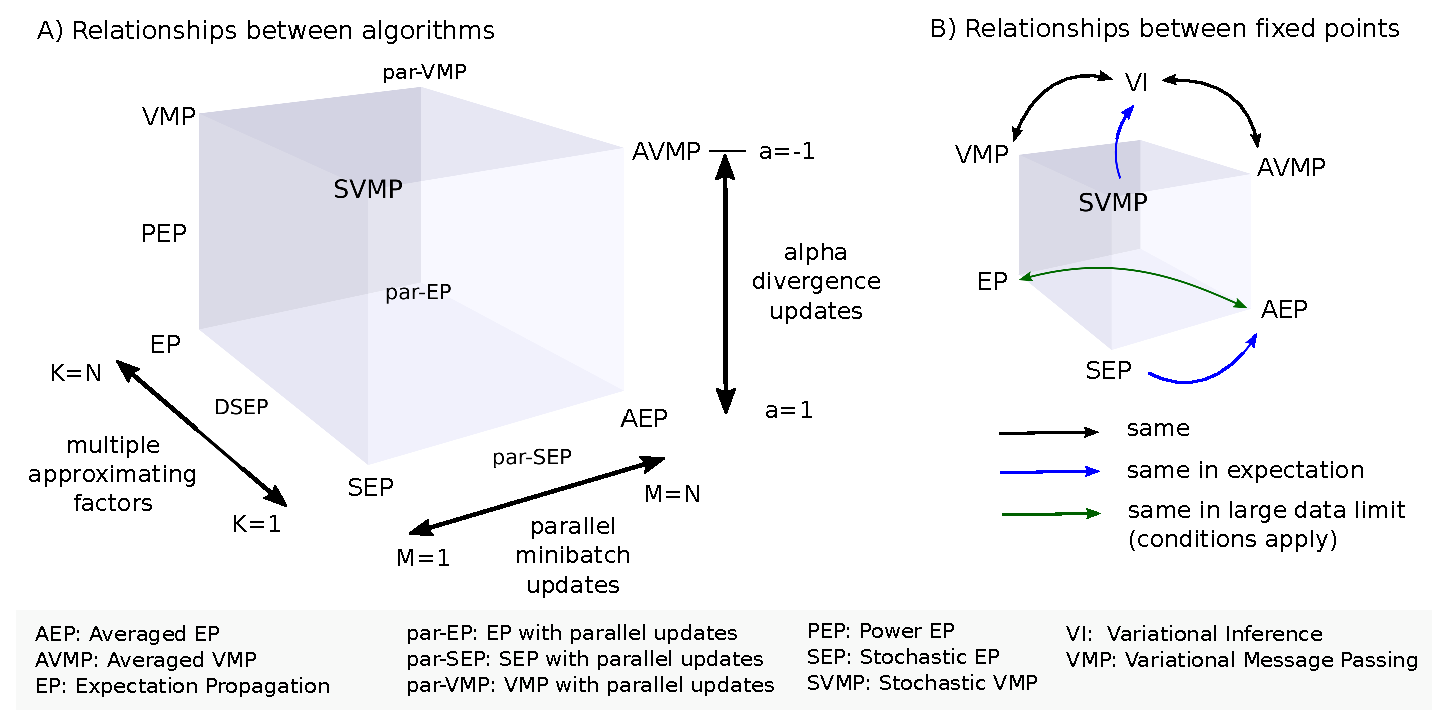
\includegraphics[height=6.5cm]{fig/relationship-algorithms.eps}%}
\caption{Relationships between algorithms. Note that care needs to be taken when interpreting the alpha-divergence as $a \rightarrow -1$ (see supplementary material).}
\label{fig:relationship-algorithms}
\end{figure}